Um den Nutzern eine ansprechende Benutzeroberfläche zu bieten, durch die der Klient über eine Schnittstelle mit dem Server kommunizieren kann und schlussendlich unsere Webseite bedienen kann, ist eine Mehrzahl an Technologien, Techstack oder Technologieinfrastruktur genannt, notwendig.

Es wurde sich für MERN entschieden, einem ausgereiften Stack bestehend aus MongoDB als Datenbank, NodeJS und Express im Backend und React im Frontend. Alle dieser Technologien verwenden die Programmiersprache JavaScript, dies erleichtert das Programmieren, da nicht zwischen den Syntaxen verschiedener Sprachen gewechselt werden muss. Auch kann der gleiche Programmiercode an verschiedenen Stellen des Projektes wiederverwendet werden, was Zeit und Kosten spart. Alle Technologien sind ausgereift und werden vielfach aktiv von führenden Technologiegiganten verwendet. Zudem wird für die Programmierschnittstelle statt einer typischen REST-API GraphQL (Graph Query Language) verwendet, welches Datenabfragen an einigen Stellen vereinfacht. Die Technologien sowie Alternativen und die Gründe zur Entscheidung werden in den folgenden Kapiteln erläutert.

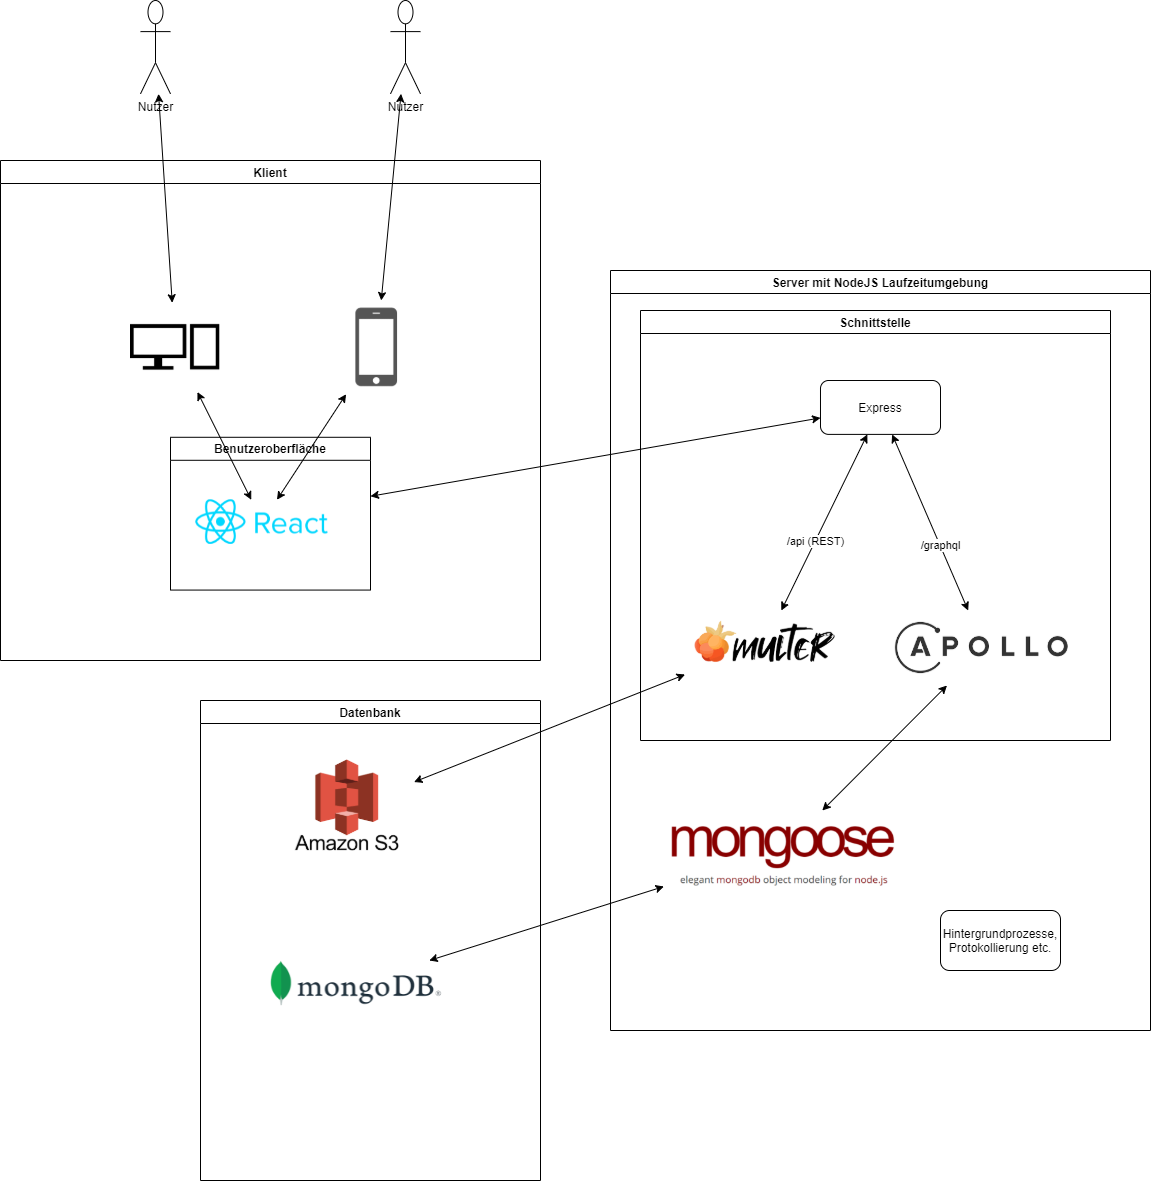
\includegraphics[width=\textwidth]{sources/MERN-Stack_Schaubild.drawio}
\begin{figure}[ht]
	\centering
	\caption{Die Interaktion der verwendeten Technologien als Schaubild}
	\label{figMERN1}
\end{figure}

Der Benutzer interagiert durch sein Endgerät mit der Webseite. Wenn die Webseite aufgerufen wird, wird zuerst durch Express anhand der Route entschieden, welche Technologie mit der Anfrage umgehen soll. Wenn es sich nicht um eine spezifische Route handelt, wird die Anfrage an React weitergeleitet und es wird eine Benutzeroberfläche bereit gestellt. Sollte der Benutzer eine Seite anfragen, auf der dynamische Inhalte angezeigt werden (zum Beispiel Nutzerprofile) oder die aus anderen Gründen eine Datenbankanbindung benötigen (zum Beispiel Anmeldung, Registrierung), wird automatisch eine Anfrage an die entsprechenden Endpunkte erstellt. In diesem Fall wird eine Anfrage an \textit{/api} oder\textit{/graphql} an Express gesendet, welches dann die Anfrage respektiv an Multer - im Fall von hochgeladenen Dateien - oder an Apollo (dem gewählten GraphQL Framework) für alle anderen Abfragen weiterleitet. Im Fall von Apollo werden die in GraphQL gestellten Anfragen in für Mongoose - dem Objektmodellierungswerkzeug für MongoDB - in verständliche Datenbankabfragen übersetzt, welche dann an die Datenbank gesendet werden. Die Daten in der Antwort werden dann wiederum in React eingefügt. Die Datenbankabfragen werden im Hintergrund ausgeführt, der Benutzer interagiert nur über die Benutzeroberfläche mit dem verwaltenden Server.

